% This file was created by matlab2tikz.
%
%The latest updates can be retrieved from
%  http://www.mathworks.com/matlabcentral/fileexchange/22022-matlab2tikz-matlab2tikz
%where you can also make suggestions and rate matlab2tikz.
%
\definecolor{mycolor1}{rgb}{0.00000,0.44700,0.74100}%
\definecolor{mycolor2}{rgb}{0.85000,0.32500,0.09800}%
\definecolor{mycolor3}{rgb}{0.92900,0.69400,0.12500}%
\definecolor{mycolor4}{rgb}{0.49400,0.18400,0.55600}%
\definecolor{mycolor5}{rgb}{0.46600,0.67400,0.18800}%
%
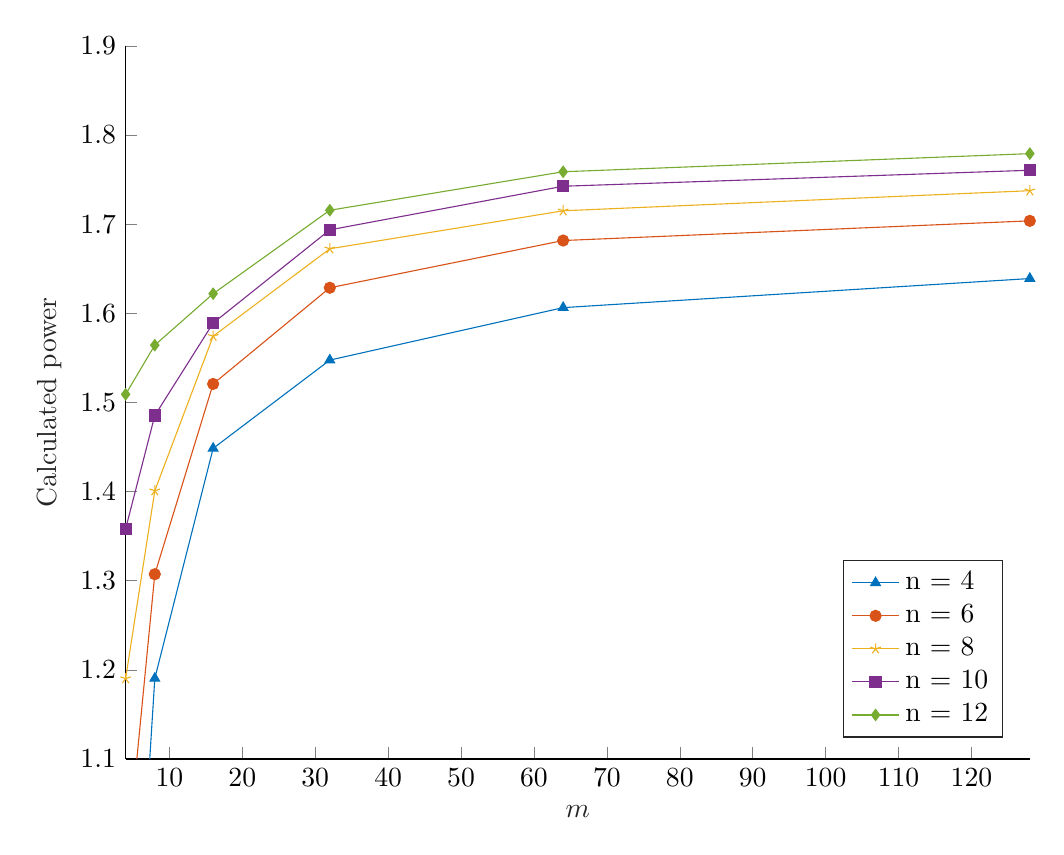
\begin{tikzpicture}

\begin{axis}[%
width=4.521in,
height=3.566in,
at={(0.758in,0.481in)},
scale only axis,
xmin=4,
xmax=128,
xlabel style={font=\color{white!15!black}},
xlabel={$m$},
ymin=1.1,
ymax=1.9,
ylabel style={font=\color{white!15!black}},
ylabel={Calculated power},
axis background/.style={fill=white},
title style={font=\bfseries},
%title={Power of m in the time complexity. On n 	imes m grid. (free slots = 0.60)},
axis x line*=bottom,
axis y line*=left,
legend style={at={(0.97,0.03)}, anchor=south east, legend cell align=left, align=left, draw=white!15!black}
]
\addplot [color=mycolor1, mark=triangle*]
  table[row sep=crcr]{%
4	0.669026765509631\\
8	1.19037285083519\\
16	1.44842455988843\\
32	1.54743567519849\\
64	1.60629928341402\\
128	1.63892960960142\\
};
\addlegendentry{n = 4}

\addplot [color=mycolor2, mark=*]
  table[row sep=crcr]{%
4	0.970440436116717\\
8	1.30727237994887\\
16	1.52068841884016\\
32	1.62857498568732\\
64	1.68156430994049\\
128	1.7036336793869\\
};
\addlegendentry{n = 6}

\addplot [color=mycolor3, mark=star]
  table[row sep=crcr]{%
4	1.19019849599422\\
8	1.40091038217518\\
16	1.57421895959424\\
32	1.672312268618\\
64	1.71493184086216\\
128	1.73745987163965\\
};
\addlegendentry{n = 8}

\addplot [color=mycolor4, mark=square*]
  table[row sep=crcr]{%
4	1.35817721613353\\
8	1.48524715774898\\
16	1.58897430870668\\
32	1.69355045147467\\
64	1.74245587066209\\
128	1.76038194217685\\
};
\addlegendentry{n = 10}

\addplot [color=mycolor5, mark=diamond*]
  table[row sep=crcr]{%
4	1.50901438516939\\
8	1.56422794761667\\
16	1.62189891981574\\
32	1.71551537332657\\
64	1.75869851092689\\
128	1.77903137048533\\
};
\addlegendentry{n = 12}

\end{axis}
\end{tikzpicture}%